\label{impl_exp}

\subsection{RMSD Benchmark}
\label{sec:RMSD}
The RMSD algorithm for the present test case represents a task for which the computational workload per frame is smaller than the I/O workload per frame (typical values $t_{\text{compute}}^{\text{frame}} = 0.09\ \text{ms}$, $t_{\text{IO}}^{\text{frame}} = 0.3\ \text{ms}$, thus $\tcomp/\tIO \approx 0.3$). 
We showed previously that the RMSD task only scaled well up to 24 cores, on a single compute node on \emph{SDSC Comet}, and \emph{TACC Stampede}, using either Dask or MPI \cite{Khoshlessan:2017ab}.

Here we focus on the MPI implementation (via \package{mpi4py} \cite{Dalcin:2011aa, Dalcin:2005aa}), in order to better understand the cause for the lack of scaling across nodes.
As in the previous work we also observed very poor strong scaling performance (Figures \ref{fig:MPIscaling}, \ref{fig:MPIspeedup} and \ref{fig:MPIscaling-Bridges} and \ref{fig:MPIspeedup-Bridges}) beyond a single node.
A more detailed analysis showed that the RMSD computation itself and to a lesser degree the I/O considered on their own scaled well beyond 50 cores (yellow and blue lines in Figure \ref{fig:ScalingComputeIO}) but the communication (red line in Figure \ref{fig:ScalingComputeIO}) and the initial file opening (gray line in Figure \ref{fig:ScalingComputeIO}) started to dominate.
Communication cost and initial time for opening the trajectory were distributed unevenly across the MPI ranks, as shown in the example in Figure \ref{fig:MPIranks}. 
The ranks that took much longer to complete than the mean execution time of all other ranks were the stragglers that hurt performance.

\subsubsection*{Identification of Scalability Bottlenecks}

In the example run in Figure \ref{fig:MPIranks}, 62 ranks out of 72 took about 60~s whereas the remaining ranks only took about 20~s. 
The detailed breakdown of the time spent on each rank (Figure \ref{fig:MPIranks}) showed that time
for the actual computation, \tcomp, was fairly constant across ranks. 
The time spent on reading data from the shared trajectory file on the Lustre file system into memory, \tIO, showed variability across different ranks. 
The stragglers, however, appeared to be defined by occasional much larger \emph{communication} times, \tcomm (line 16 in Algorithm \ref{alg:RMSD}), which were on the order of 30~s in this example, and by larger times to initially open the trajectory (line 2 in Algorithm \ref{alg:RMSD}).
For other ranks, \tcomm varied across different ranks and was barely measurable for a few ranks.
Although the data in Figure \ref{fig:MPIranks} only represented one example and in other instances perhaps only ten ranks were stragglers, the overall picture was confirmed by the averages over five independent repeats and all ranks (Figure \ref{fig:ScalingComputeIO}).
This initial analysis indicated that communication is a major issue that prevents good scaling beyond a single node, but the problems related to file I/O also played an important role in limiting performance.

\begin{figure}
\centering
\begin{subfigure}{.4\textwidth}
  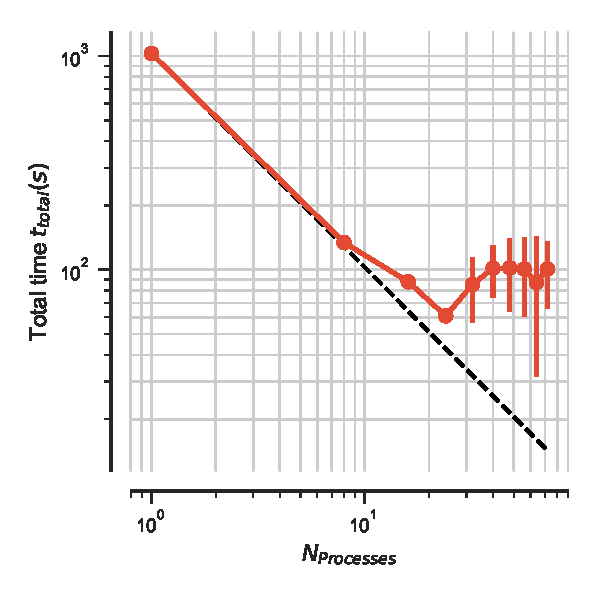
\includegraphics[width=\linewidth]{figures/main-RMSD-t_total.pdf}
  \captionsetup{format=hang}
  \caption{Scaling total (five repeats)}
  \label{fig:MPIscaling}
\end{subfigure}
\hfill
\begin{subfigure}{.4\textwidth}
  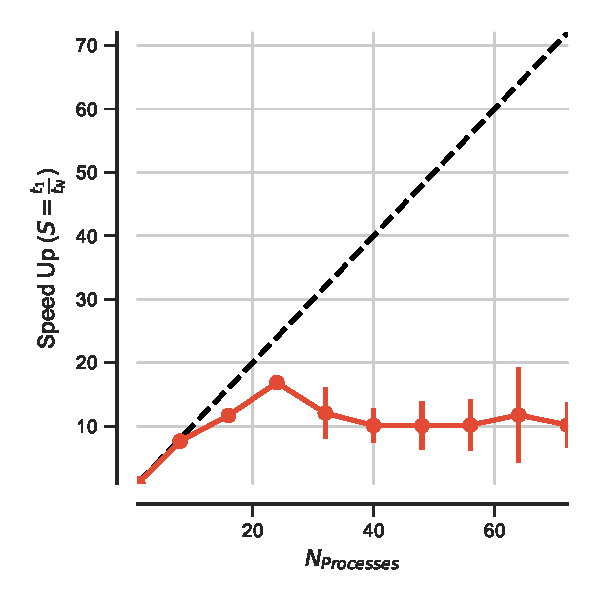
\includegraphics[width=\linewidth]{figures/main-RMSD-speed_up.pdf}
  \captionsetup{format=hang}
  \caption{Speed-up (five repeats)}
  \label{fig:MPIspeedup}
\end{subfigure}
\bigskip

\begin{subfigure}{.4\textwidth}
  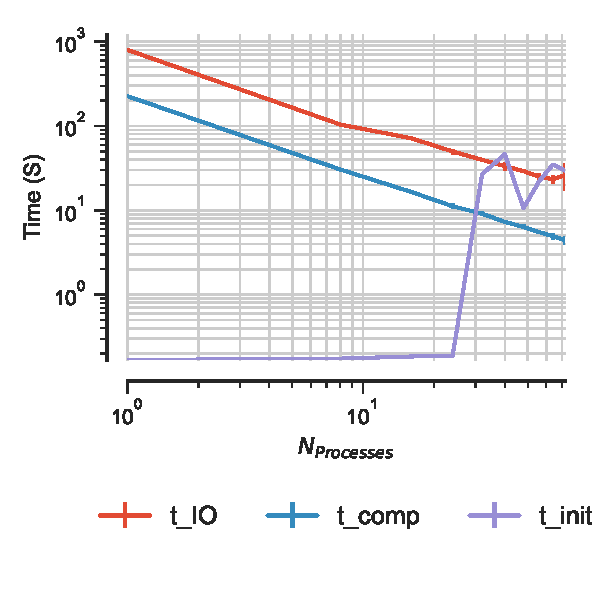
\includegraphics[width=\linewidth]{figures/main-RMSD-time_comp_IO_comparison.pdf}
  \captionsetup{format=hang}
\caption{Scaling for different components (five repeats)}
\label{fig:ScalingComputeIO}
\end{subfigure}
\hfill
\begin{subfigure} {.5\textwidth}
  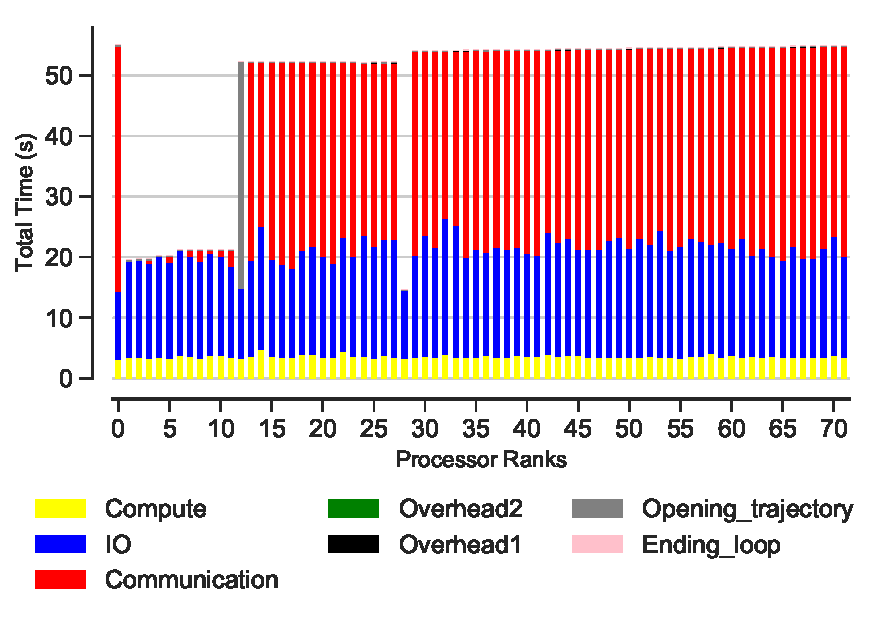
\includegraphics[width=\linewidth]{figures/main-RMSD-BarPlot-rank-comparison_72_5.pdf}
  \captionsetup{format=hang}
  \caption{Time comparison on different parts of the calculations per MPI rank (example)}
  \label{fig:MPIranks}
\end{subfigure}

\caption{Performance of the RMSD task (I/O-bound with $\tcomp/\tIO \approx 0.3$) with MPI on \emph{SDSC Comet}.
Results were communicated back to rank 0. Five independent repeats were performed to collect statistics. (a-c) The error bars show
standard deviation with respect to mean. (d) Compute \tcomp, IO \tIO, communication \tcomm, ending the for loop \text{$t_{\text{end\_loop}}$},
  opening the trajectory \text{$t_{\text{opening\_trajectory}}$}, and overheads \text{$t_{\text{overhead1}}$}, \text{$t_{\text{overhead2}}$} per MPI rank (see Table \ref{tab:notation} for the definition).
These are data from one run of the five repeats. MPI ranks 0, 12--27 and 29--72 are stragglers. \textbf{Note:} In serial, there is no communication.}
\label{fig:MPIwithIO}
\end{figure} 

\subsubsection*{Influence of Hardware}
We ran the same benchmarks on multiple HPC systems (XSEDE resources \emph{PSC Bridges} (Fig.~\ref{fig:MPIwithIO-Bridges}) and \emph{LSU SuperMIC} (Fig.~\ref{fig:MPIwithIO-SuperMIC})) and observed the occurrence of stragglers, in a manner very similar to the results already described for \emph{SDSC Comet}.
There was no clear pattern in which certain MPI ranks would always be a straggler and neither could we trace stragglers to specific cores or nodes. 
Therefore, the phenomenon of stragglers in the RMSD test appeared to be independent from the cluster and thus the underlying hardware.


\subsection{Effect of \tcomp/\tIO on Performance}
\label{bound}

The results in the previous section indicated communication and I/O to be two important factors that appeared to correlate with stragglers. 
In order to better characterize the RMSD task, we computed the ratio between the time to complete the computation and the time spent on I/O, $\tcomp/\tIO = 0.3$, and found that this task was I/O bound, i.e.,
\begin{gather*}
  \frac{\tcomp}{\tIO} \ll 1.
\end{gather*}
For such a compute-bound task we were not able to achieve good scaling beyond a single node. 
We hypothesized that decreasing the relative I/O load with respect to the compute load would also reduce the impact of stragglers by interleaving I/O with longer periods of computation and thus reducing the impact of I/O contention.
We therefore set out to measure compute bound tasks, i.e.\ ones with
\begin{gather*}
  \frac{\tcomp}{\tIO} \gg 1.
\end{gather*}
To measure the effect of the $\tcomp/\tIO$ ratio on performance but leaving other parameters the same, we artificially increased the computational load by repeating the same RMSD calculation (line 10, algorithm \ref{alg:RMSD}) 40, 70 and 100 times in a loop, resulting in forty-fold (``$40\times$''), seventy-fold (``$70\times$''), and one hundred-fold (``$100\times$'') load increases.


\subsubsection{Effect of Increased Compute workload for RMSD Task}

The increased computational workloads corresponded to $\tcomp/\tIO$ ratios of 11, 19, 27 respectively as shown in Table \ref{tab:load-ratio}.
These generally agreed with the simple theoretical prediction in Table \ref{tab:load-ratio} that the $\tcomp/\tIO$ ratio for the higher workloads (with factor $X$) should be $X$ times the $\tcomp/\tIO$ for the $1\times$ workload because on average the I/O workload of each rank is $N_{\text{b}} \times \tIO $ (where $N_{\text{b}} = N_{\text{frames}}^{total}/N$ is the number of frames per trajectory block, i.e., the number of frames processed by each MPI rank for $N$ processes), which is independent of $X$, while the workload for the computation is $X \times N_{\text{b}} \times \tcomp$, and hence the ratio is $X \times \tcomp/\tIO$.

\begin{table}[ht!]
\centering
\begin{tabular}{rrrrr}
  \toprule
  \bfseries\thead{Workload} &  \bfseries\thead{$\tcomp$} &  \bfseries\thead{$\tIO$}
  & \multicolumn{2}{c}{\bfseries\thead{$\tcomp/\tIO$}}\\
  & & & \thead{measured} & \thead{theoretical}\\
  \midrule
    $1\times$   &   226 & 791 &  0.29 &   \\  
    $40\times$  &  8655 & 791 & 11   & 11\\    
    $70\times$  & 15148 & 791 & 19   & 20\\  
    $100\times$ & 21639 & 791 & 27   & 29\\  
  \bottomrule
\end{tabular}
\caption[Change in load-ratio with RMSD workload]{Change in $\tcomp/\tIO$ ratio with change in the RMSD workload.
  The RMSD workload was artificially increased in order to examine the effect of compute to I/O ratio on the performance.
  The reported compute and I/O time were calculated based on the serial version using one core and used to calculate the measured $\tcomp/\tIO$.
  The theoretical $\tcomp/\tIO$ (see text) is provided for comparison.}
\label{tab:load-ratio}
\end{table}

We performed this experiment to show the effect of the $\tcomp/\tIO$ ratio on performance (Figure \ref{fig:tcomp_tIO_effect}).
As the $\tcomp/\tIO$ ratio increased, speed-up and performance improved and 
showed overall better scaling than the I/O-bound workload, i.e. $1\times$ RMSD (Figure \ref{fig:S1_tcomp_tIO_effect}).
When $\tcomp/\tIO$ ratio increased, the RMSD calculation consistently scaled up to larger numbers of cores ($N=56$ for $70\times$ RMSD).
Figures \ref{fig:S2_tcomp_tIO_effect} and \ref{fig:E_tcomp_tIO_effect} show that speed-up and efficiency approach their ideal value for each processor count with increasing $\tcomp/\tIO$ ratio.

\begin{figure}[ht!]
\centering
\begin{subfigure} {.3\textwidth}
  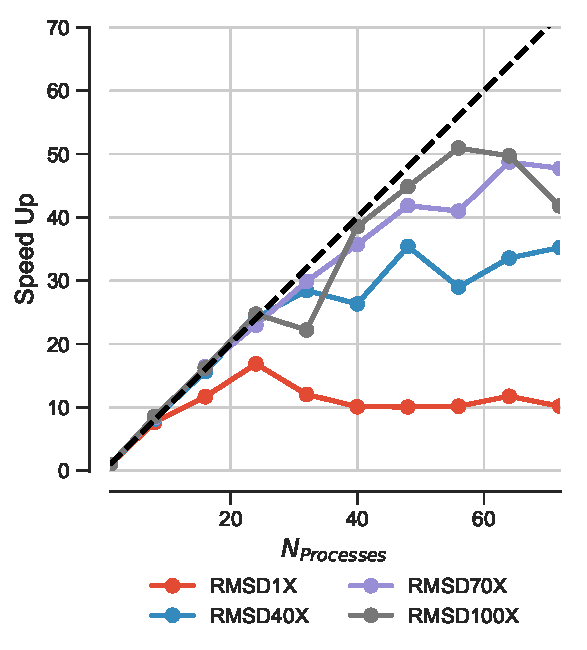
\includegraphics[width=\linewidth]{figures/Compute_to_IO_ratio_on_performance_2d_v17.pdf}
  \caption{Speed-Up}
  \label{fig:S1_tcomp_tIO_effect}
\end{subfigure}
\hfill
\begin{subfigure}{.3\textwidth}
  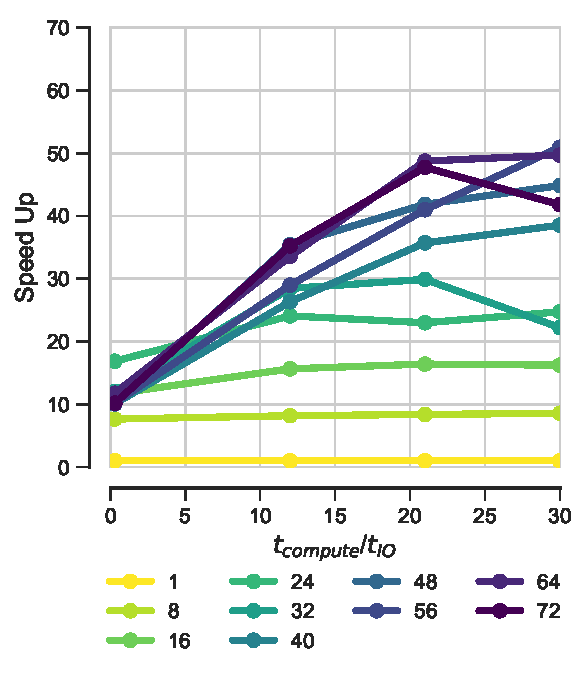
\includegraphics[width=\linewidth]{figures/Compute_to_IO_ratio_on_performance_2d_2_v17.pdf}
  \caption{Speed-Up}
  \label{fig:S2_tcomp_tIO_effect}
\end{subfigure}
\hfill
\begin{subfigure}{.3\textwidth}
  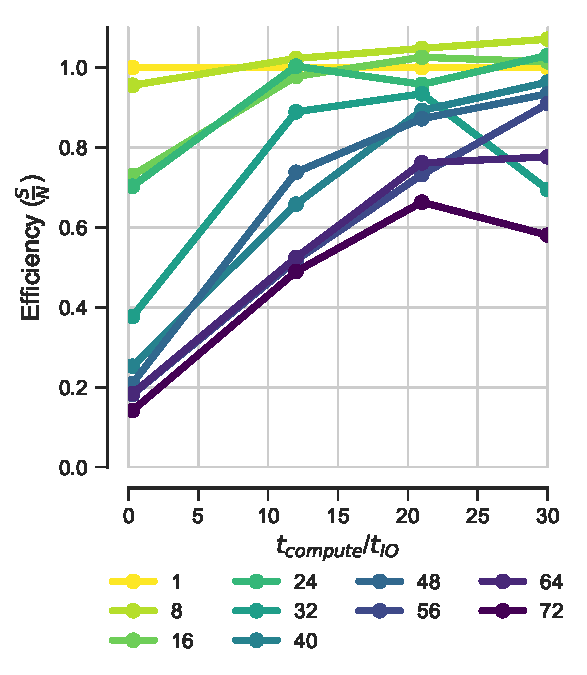
\includegraphics[width=\linewidth]{figures/Compute_to_IO_ratio_on_performance_2d_3_v17.pdf}
  \caption{Efficiency}
  \label{fig:E_tcomp_tIO_effect}
\end{subfigure}
%
\caption{Effect of \text{$\tcomp/\tIO$} ratio on performance of the RMSD task with MPI performed on \emph{SDSC Comet}. We tested performance for $\tcomp/\tIO$ ratios of 0.3, 11, 19, 27 \obnote{FIX THESE GRAPHS, should correspond to measured numbers in Table \protect\ref{tab:load-ratio}, see \protect\href{https://github.com/hpcanalytics/paper-hpc-py-parallel-mdanalysis/issues/8}{issue \#8}}
which correspond to $1\times$ RMSD, $40\times$ RMSD, $70\times$ RMSD, and $100\times$ RMSD respectively. (a) Effect of \tcomp/\tIO on the Speed-Up
(b) Change in the Speed-Up with respect to $\tcomp/\tIO$ for different processor counts (c) Change in the efficiency with respect to $\tcomp/\tIO$ for different processor counts}
\label{fig:tcomp_tIO_effect}
\end{figure}

Even for moderately compute-bound workloads such as the $40\times$ and $70\times$ RMSD tasks, increasing the computational workload over I/O reduced the impact of stragglers even though they still contribute to large variations in timing across different ranks and thus irregular scaling due to the fluctuations.

\subsubsection{I/O leads to stragglers}

When we removed I/O from the RMSD calculation by generating comparable input data randomly, performance significantly improved (Figure \ref{fig:MPIwithoutIO}).
Given the results for the RMSD algorithm (Algorithm \ref{alg:RMSD}) and $X\times$ RMSD (Figure \ref{fig:tcomp_tIO_effect}) and RMSD without I/O (Figure \ref{fig:MPIwithoutIO}) it seems possible that MPI competes with Lustre on the same network interface, which would explain why communication appears to be primarily a problem in the presence of I/O when \tcomp/\tIO is small.
In fact, these results suggest that decreasing the I/O load relative to the compute load should open up the network for communication.
This can be confirmed from other previous studies as well \cite{VMD2013, Kevin2018}. % TODO: cite 2018 CPPC paper 

\subsection{Communication Cost and Application of Global Arrays}
\label{Global-Array}
As discussed in the previous sections, Figure \ref{fig:MPIranks}, for small \tcomp/\tIO, communication acts as the scalability bottleneck. 
When the processes communicated result arrays back to the master process (rank 0), some processes took much longer as compared to other processes. 
Here we investigate strategies to reduce communication cost. 

We used Global Arrays (GA) \cite{GA, GAiN} instead of collective communication in MPI and examined the change in the performance. 
In GA, we define one large RMSD array called \emph{global array}, and each MPI rank updates its associated block in the global RMSD array using \text{ga\_put()}. 
At the end, when all the processes exit \text{block\_rmsd()} function and update their local block in the global array, rank 0 will access the whole global array using \text{ga\_access()}.
In GA, the time for communication is \text{$t_{\text{ga\_put()}}+t_{\text{ga\_access()}}$}.
Given the speed up plots (Figure \ref{fig:MPIspeedup-ga4py}) and total time scaling (Figure \ref{fig:MPIscaling-ga4py}) Global Arrays improves strong scaling performance.
Although, communication time has significantly decreased using Global Arrays (compare Figure \ref{fig:MPIranks-ga4py} to Figure \ref{fig:MPIranks}),
the existing variation in the dominant I/O part of the calculation plus two delayed MPI ranks due to the delay in opening the trajectory would still prevent ideal scaling (Figure \ref{fig:ScalingComputeIO-ga4py}).
These slow processes due to opening the trajectory take about 50~s, which are slower than the mean execution time of all ranks, i.e. 17~s. 
This figure shows only one repeat out of the five that we performed for our benchmark study. 
In fact, although communication time significantly reduced using Global Arrays, scaling is still far from ideal as a result of slow processes due to I/O variation and the delay in opening the trajectory.
\obnote{If these are not "typical data" then we should show more typical one. On the other hand, scaling is poor at high N, so clearly there are some stragglers even in the other cases. If it's not trajectory opening, then what are these stragglers?}
\mknote{All other repeats are showing the similar behavior. I put them in a zip file and pushed in the repository. But opening the trajectory is part of I/O and file access. Is not it?}

\begin{figure}[ht!]
\centering
\begin{subfigure}{.4\textwidth}
  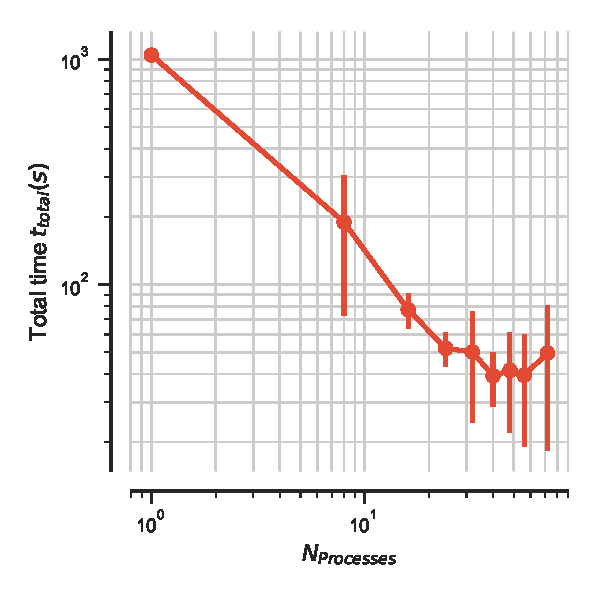
\includegraphics[width=\linewidth]{figures/RMSD-ga4py-t_total.pdf}
  \captionsetup{format=hang}
  \caption{Scaling total}
  \label{fig:MPIscaling-ga4py}
\end{subfigure}
\hfill
\begin{subfigure}{.4\textwidth}
  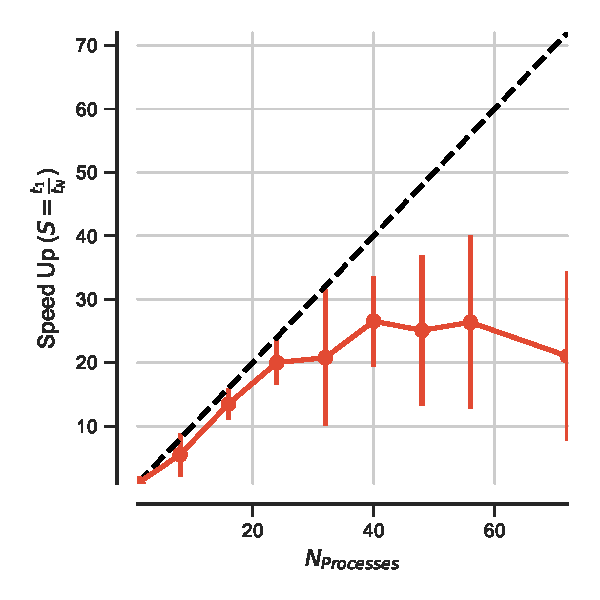
\includegraphics[width=\linewidth]{figures/RMSD-ga4py-speed_up.pdf}
  \captionsetup{format=hang}
  \caption{Speed-up}
  \label{fig:MPIspeedup-ga4py}
\end{subfigure}
\bigskip

\begin{subfigure}{.4\textwidth}
  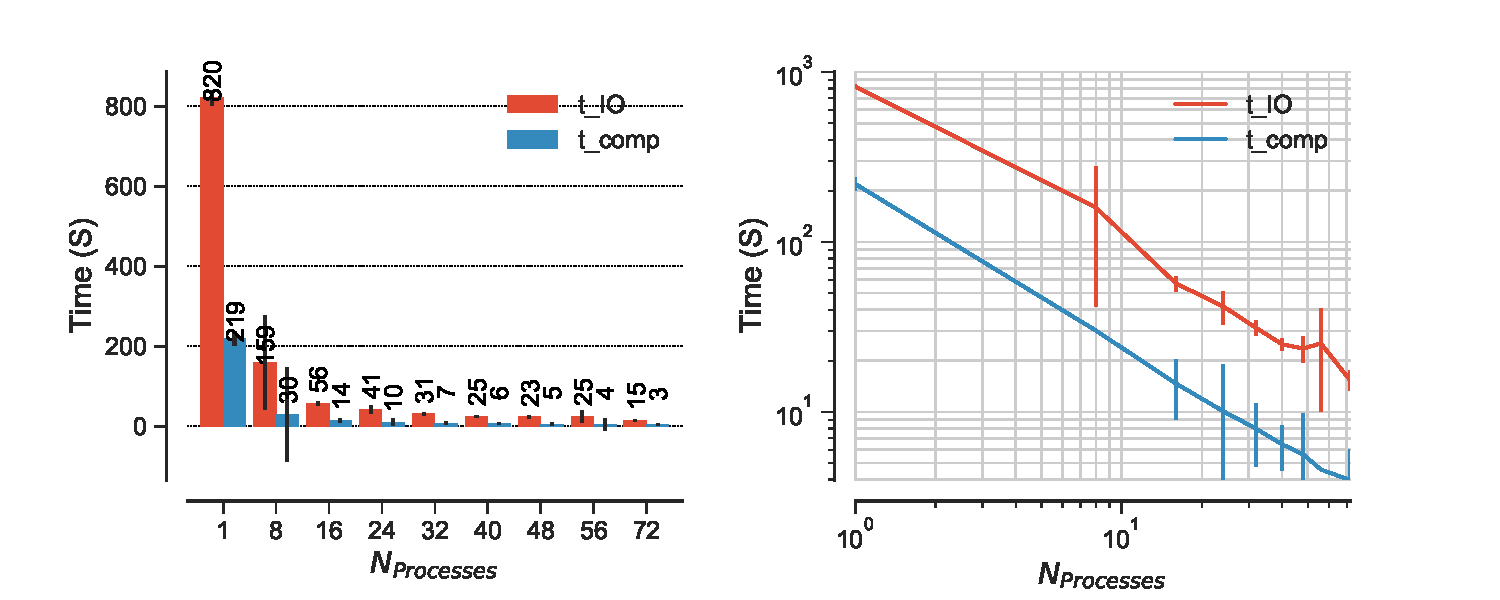
\includegraphics[width=\linewidth]{figures/RMSD-ga4py-time_IO_comparison.pdf}
  \captionsetup{format=hang}
\caption{Scaling for different components}
\label{fig:ScalingComputeIO-ga4py}
\end{subfigure}
\hfill
\begin{subfigure} {.5\textwidth}
  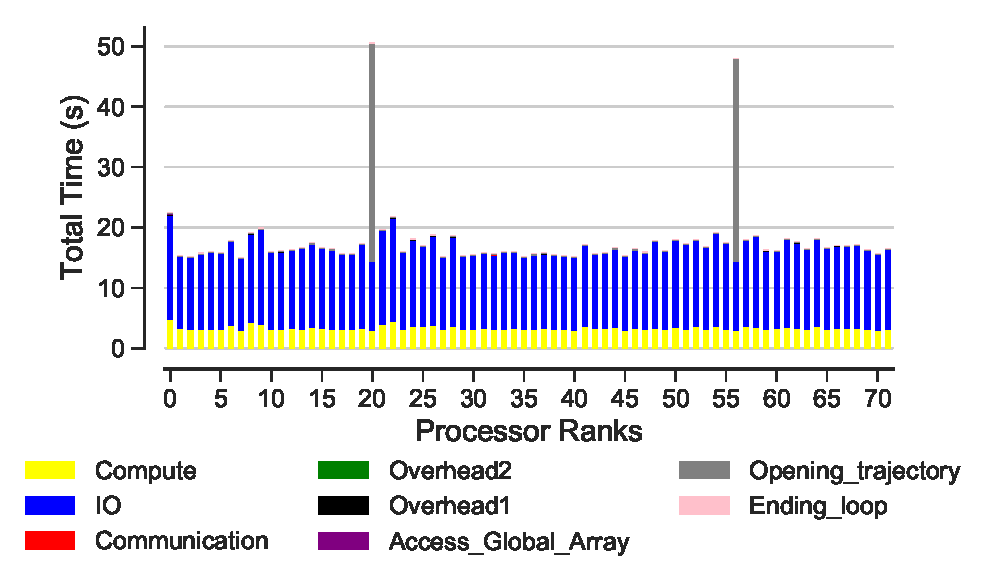
\includegraphics[width=\linewidth]{figures/RMSD-ga4py-BarPlot-rank-comparison_72_1.pdf}
  \captionsetup{format=hang}
  \caption{Time comparison on different parts of the calculations per MPI rank}
  \label{fig:MPIranks-ga4py}
\end{subfigure}

\caption{Performance of the RMSD task with MPI using Global Arrays ($\tcomp/\tIO \approx 0.3$) on SDSC Comet.
All ranks update the Global Arrays (\text{ga\_put()}) and rank 0 accesses the whole RMSD array through the global memory address (\text{ga\_get()}) (communications included).
Five repeats were performed to collect statistics. (a-c) The error bars show standard deviation with respect to mean. 
(d) Compute \tcomp, IO \tIO, communication \tcomm, access to the whole Global Arrays by rank 0, \text{$t_{\text{Access\_Global\_Array}}$}, ending the for loop \text{$t_{\text{end\_loop}}$},
  opening the trajectory \text{$t_{\text{opening\_trajectory}}$}, and overheads \text{$t_{\text{overhead1}}$}, \text{$t_{\text{overhead2}}$} per MPI rank (See Table \ref{tab:notation} for the definition). 
  This is typical data from one run of the 5 repeats. MPI ranks 20 and 56 are stragglers, i.e., 
their total time far exceeds the mean of the all ranks. \textbf{Note:} In serial, there is no communication.}
\label{fig:MPIwithIO-ga4py}
\end{figure}

\subsection{I/O Cost}
\label{I/O}

We previously showed that the I/O system can have a large effect on the parallel performance of the RMSD task \cite{Khoshlessan:2017ab} and the results above show that in the I/O-bound problem stragglers prevent us from effectively utilizing HPC resources (see Figure \ref{fig:ScalingComputeIO}, for $\tcomp/\tIO \approx 0.3$).
The root cause for this behavior is not immediately obvious but by analyzing the flow of data in the context of the Lustre filesystem on which the trajectory files are stored  we can get a sense of possible problem areas.

In MDAnalysis, individual trajectory frames are loaded into memory, which ensures that even systems with tens of millions of atoms can be efficiently analyzed on resources with moderate RAM sizes. 
The test trajectory (file size 30 GB) has $2,512,200$ frames in total so each frame is about 0.011 MB in size.
With $\tIO \approx 0.3~\text{ms}$ per frame, the data are ingested at a rate of about $40$~MB/s for a single process.
For 24 MPI ranks (one \emph{SDSC Comet} node), the aggregated reading rate would be about 1 GB/s, which seems to be well within the the available bandwidth of 56 Gb/s of the Infiniband network interface that serves the Lustre file system.
The default Lustre stripe size value is 1~MB, i.e., the amount of contiguous data stored on a single Lustre object storage target (OST).
Each I/O request reads a single Lustre stripe but because the I/O size (0.011~MB) is smaller than the stripe size, many of these I/O requests are likely just accessing the same stripe on the same OST but nevertheless have to acquire a new reading lock for each request.
Such a situation can incur locking overheads \cite{optimize_lustre}, although it is not clear how severely the performance is generally affected in such cases.
More generally, contention for the interconnect between OSTs and compute nodes due to MPI communication may lead to variable performance in I/O measurements \cite{Mache:2005aa}.
Conversely, our data suggest that naive single-shared-file I/O on Lustre can negatively affect the MPI communication, even at moderate numbers (tens to hundreds) of concurrent requests.

In order to improve performance, we therefore need to employ strategies to avoid the competition over file access across different ranks when the \tcomp/\tIO ratio is small.
To this end we experimented with two different ways for reducing the I/O cost:
splitting the trajectory file into as many segments as the number of processes, thus using file-per-process access, and using the HDF5 file format together with MPI-IO parallel reads instead of the XTC trajectory format.
We discuss these two approaches and the resulting performance improvements in detail in the following sections.

\subsubsection{Splitting the Trajectories}
\label{splitting-traj}
In all the previous benchmarks all processes were using a shared trajectory file.
Here, we propose splitting our trajectory file into as many trajectory segments as the number of processes.
Subfiling, is a mechanism that is previously used for splitting a large multi-dimensional global array to a number of smaller subarrays, each saved in a separate file. 
This scheme reduces the file system control overhead by decreasing the number of processes concurrently accessing a shared file \cite{scalable-IO, scalable-IO1}.
Subfiling is known to improve programming flexibility and performance of parallel shared-file I/O. 
In the present study, we employ a similar approach through which, if we have $N$ processes, the trajectory file is split into $N$ segments and each segment will have $N_{b}$ frames in it. 
In fact, each process will have access to its own trajectory segment and there should be no competition for file accesses. 
For reference, we benchmarked the necessary time for splitting the trajectory using different number of processes (Table \ref{tab:timing-splitting}).

\subsubsection*{Performance without Global Arrays}
We ran a benchmark up to 8 nodes (192 cores) and, we observed rather better scaling behavior with efficiencies above 0.6 (Figure \ref{fig:MPIscaling-split} and \ref{fig:MPIspeedup-split}) with the delay time for stragglers reduced from 65 s to about 10 s for 72 processes. 
However, scaling is still far from ideal due to communication. 
Although, the delay due to communication was much smaller as compared to Parallel RMSD with shared-file I/O (Compare Figure \ref{fig:MPIranks-split} ($\tcomm^{\text{Straggler}} \gg \tcomp+\tIO$) to Figure \ref{fig:MPIranks} ($\tcomm^{\text{Straggler}} \approx \tcomp+\tIO$)), it is still delaying several processes and as a result led to longer job completion time (Figure \ref{fig:MPIranks-split}). 
These delayed tasks impacted performance and as a result speed-up was far from ideal (Figure \ref{fig:MPIspeedup-split}).

\begin{figure}[ht!]
\centering
\begin{subfigure}{.32\textwidth}
  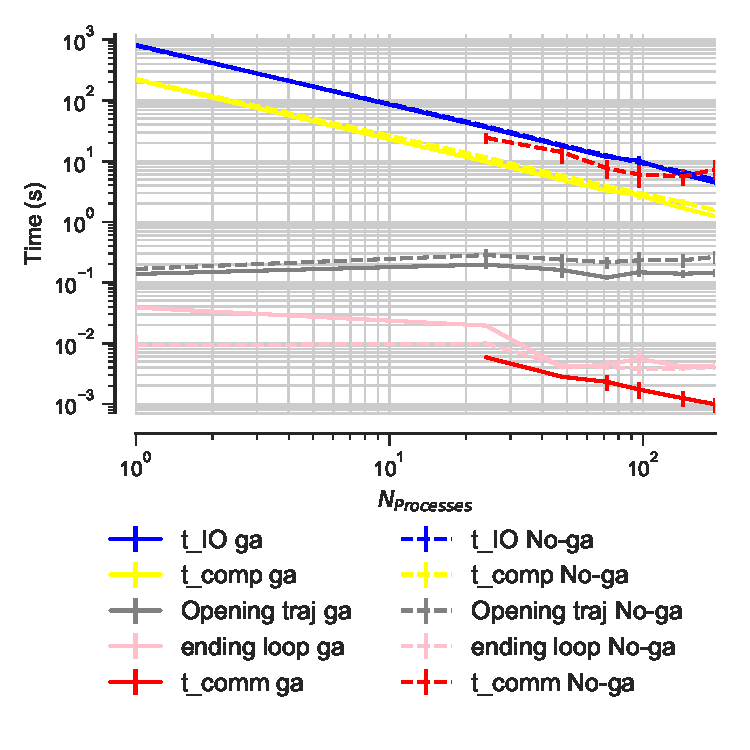
\includegraphics[width=\linewidth]{figures/Comparison_IO_compute_scaling_traj_splitting.pdf}
  \captionsetup{format=hang}
  \caption{Scaling for different components}
  \label{fig:ScalingComputeIO-split}
\end{subfigure}
\hfill
\begin{subfigure}{.3\textwidth}
  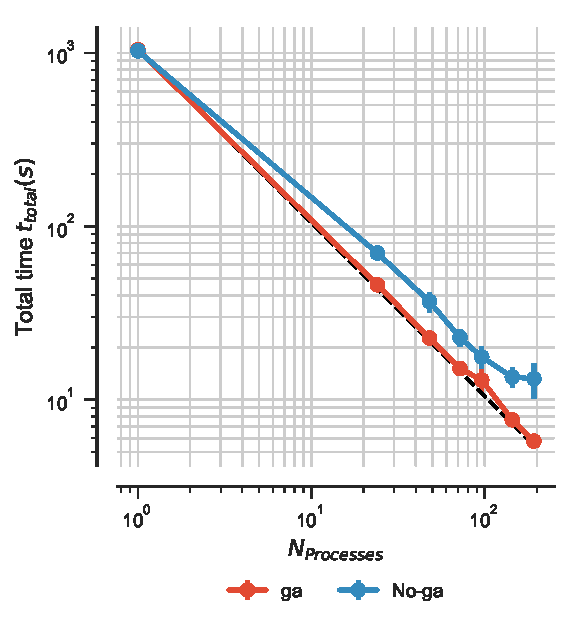
\includegraphics[width=\linewidth]{figures/Comparison_tot_time_traj_splitting.pdf}
  \caption{Scaling total}
  \label{fig:MPIscaling-split}
\end{subfigure}
\hfill
\begin{subfigure}{.3\textwidth}
  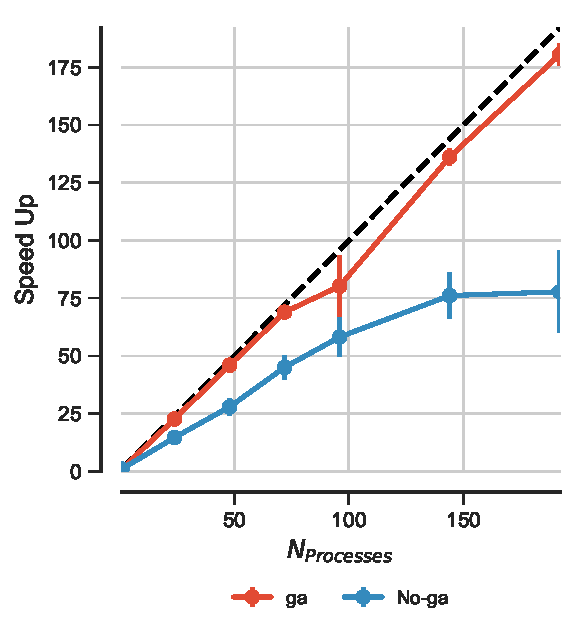
\includegraphics[width=\linewidth]{figures/Comparison_Speed_UP_traj_splitting.pdf}
  \captionsetup{format=hang}
  \caption{Speed-up}
  \label{fig:MPIspeedup-split}
\end{subfigure}
\bigskip

\begin{subfigure} {.45\textwidth}
  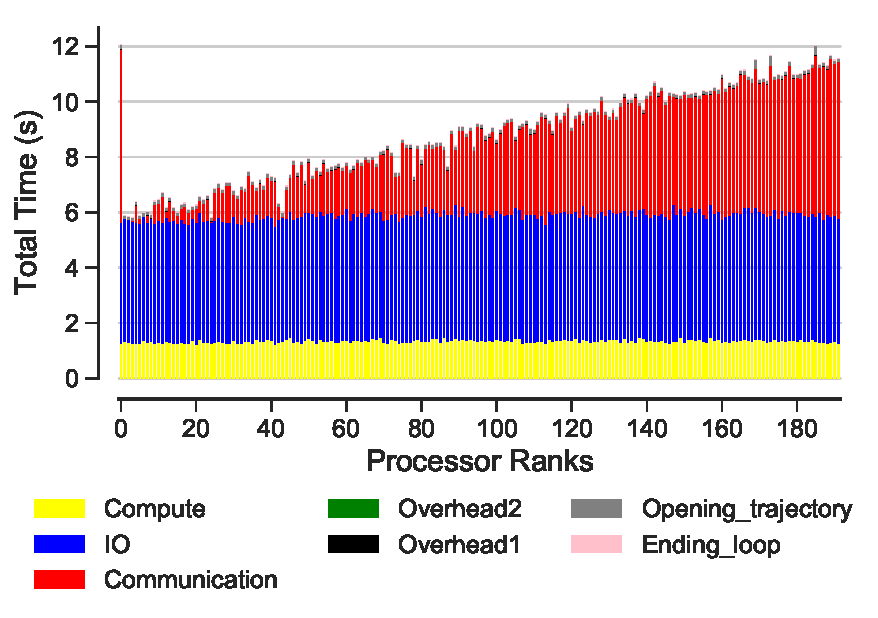
\includegraphics[width=\linewidth]{figures/split-BarPlot-rank-comparison_192_5.pdf}
  \captionsetup{format=hang}
   \caption{Time comparison on different parts of the calculations per MPI rank without Global Arrays}
  \label{fig:MPIranks-split}
\end{subfigure}
\hfill
\begin{subfigure} {.5\textwidth}
  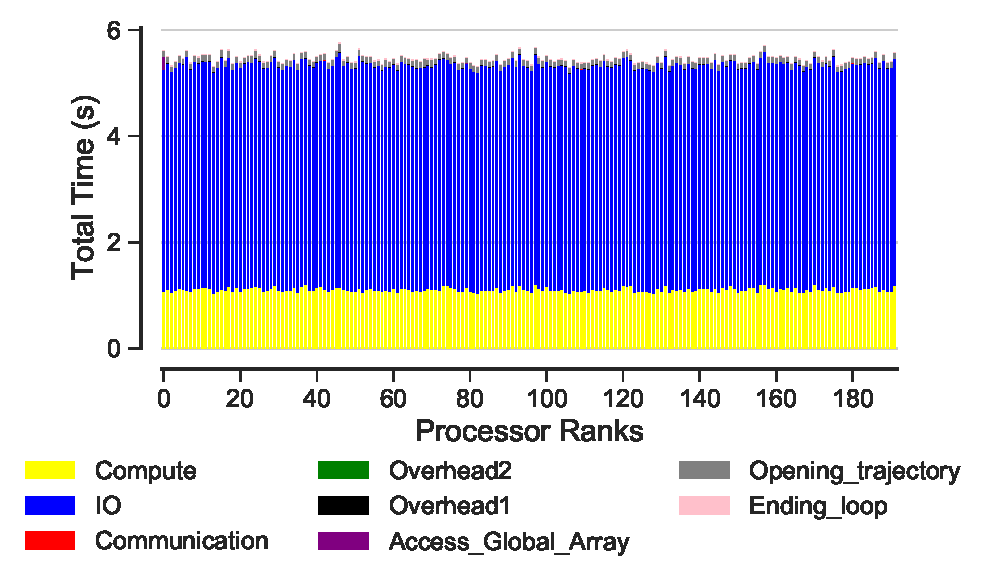
\includegraphics[width=\linewidth]{figures/split-ga-BarPlot-rank-comparison_192_5.pdf}
  \captionsetup{format=hang}
  \caption{Time comparison on different parts of the calculations per MPI rank using Global Arrays}
  \label{fig:MPIranks-split-ga}
\end{subfigure}

\caption{Comparison on the performance of the RMSD task with MPI when the trajectories are split using Global Arrays and without Global Arrays (\text{$\tcomp/\tIO \approx 0.3$}) on SDSC Comet.
In case of Global Arrays, all ranks update the Global Arrays (\text{ga\_put()}) and rank 0 accesses the whole RMSD array through the global memory address (\text{ga\_get()}).
Five repeats were performed to collect statistics. (a) Compute \& I/O scaling versus number of processes (b) Total time scaling versus number of processes (c) Speed-up (a-c) The error bars show standard deviation with respect to mean. (d-e) Compute \tcomp, IO \tIO, communication \tcomm, access to the whole Global Arrays by rank 0, \text{$t_{\text{Access\_Global\_Array}}$}, ending the for loop \text{$t_{\text{end\_loop}}$},
  opening the trajectory \text{$t_{\text{opening\_trajectory}}$}, and overheads \text{$t_{\text{overhead1}}$}, \text{$t_{\text{overhead2}}$} per MPI rank (See Table \ref{tab:notation} for the definition). When Global Arrays is not used, the performance is affected due to the non-uniform communication time across different ranks. However, when Global Arrays is used communication time has significantly reduced and scaling is close to ideal. \textbf{Note:} In serial, there is no communication.}
\label{fig:MPIwithIO-split}
\end{figure}

\subsubsection*{Performance using Global Arrays}
\gpnote{This is very confusing. In a previous paragraph you say that GA passes data over the IB network. Here you say there is no congestion? Don't they, MPI communication, MPI I/O, and GA communication, use the same network? Also, I do not think you have the data to support that clearly, unless you know how many Bytes are moved around, how many packets and their type. If that is the case include it. Or are you using the Local filesystem on the nodes and IO has nothing to do with the IB?}
\mknote{I think there is something different in the way GA use IB that when we use GA there is no contention. That is mainly because there is no synchronization and that reduces the traffic a lot. GA uses IB but the way it uses is very different from MPI Gather. it defines a pointer and that is very different from what happens in MPI for communication.}
\gpnote{So there are no similarities between GA communication and asynchronous MPI communication? Asynchronous MPI communication does not block anything and there is no need for synchronization when done correctly. It is still confusing for me at least.}\mknote{No,  there are no similarities. MPI.Gather is collective communication and collective communications are blocking in MPI, right?}\gpnote{For synchronous, yes you are right. I am asking about asynchronous MPI communication.}\mknote{Maybe using Isend and Ireceive can be helpful but I do not think it will be comparable with GA. DO you volunteer to give it a shot and replace \text{mpi.Gather} with asynchronous communication and run it so that we can compare with GA?}
Previously, we showed that Global Arrays significantly reduces the communication cost (Section \ref{Global-Array}). 
We want to examine effect of splitting the trajectory file and using Global Arrays on the performance.
Again, we ran our benchmark up to 8 nodes (192 cores) and observed near ideal scaling behavior with efficiencies above 0.9 (Figure \ref{fig:MPIscaling-split} and \ref{fig:MPIspeedup-split}) with no straggler tasks (Figure \ref{fig:MPIranks-split-ga}).  
The present results suggest that contention for file access impacts performance. 

\subsection{Effect of \tcomp/\tcomm on Performance}
\obnote{Analyze the RMSD with different load. See if t\_comp/t\_comm is also important in that case. Can you still draw the same conclusions?}
\mknote{What do you mean by different loads? tcomp/tio is constant for all number of processes and as a result we were able to see the changes with the change in the ratio. 
tcomp/tcomm is not constant with number of processes (fig 5). A better experiment would be to change size of the arrays to be communicated for RMSD 100X for example and evaluate performance. If you agree with that let me know and I wlll go ahead and run those cases.}
In addition to the compute to I/O ratio we define another important performance parameter called compute to communication ratio.
Based on the results shown in the section \ref{I/O}; although we overcame the I/O effect by splitting the trajectory, scaling is still far from ideal without Global Arrays.
This means that the task remains communication bound (Figure \ref{fig:MPIwithIO-split}). 
When the task is communication bound, i.e.,

\begin{gather*}
  \frac{t_{\text{comp}}}{t_{\text{comm}}} \ll 1.
\end{gather*}

If the computational load is more than communication load then the work became compute bound, i.e.,

\begin{gather*}
  \frac{t_{\text{comp}}}{t_{\text{comm}}} \gg 1.
\end{gather*}

Figure \ref{fig:tcom_tcomm_effect} shows the relationship of performance with \tcomp/\tcomm ratio.
When \tcomp/\tcomm ratio is higher, performance is better even if communication time is larger (Figure \ref{fig:tcomp_tcomm_ratio} and Figure \ref{fig:S2_tcomp_tIO_effect}).
Although, there are stragglers due to communication, their effect on performance is not crucial mainly because compute to communication ratio is very large. 
We therefore, conclude that higher compute to communication loads would lead to better performance. 

It should be noted that within one node, communication is not usually a problem because of the shared memory environment. 
As a result, communication time would not be problematic even if compute to communication ratio is small (Figure \ref{fig:tcomp_tcomm_ratio}, 1-24 cores represent a single compute node on SDSC Comet).
However, beyond a single node, communication overhead becomes a bottleneck and effect of \tcomp/\tcomm becomes very important (Figure \ref{fig:tcomp_tcomm_ratio}, 24-72 cores represent multiple compute nodes on SDSC Comet).

\begin{figure}[ht!]
\centering
\begin{subfigure}{.4\textwidth}
  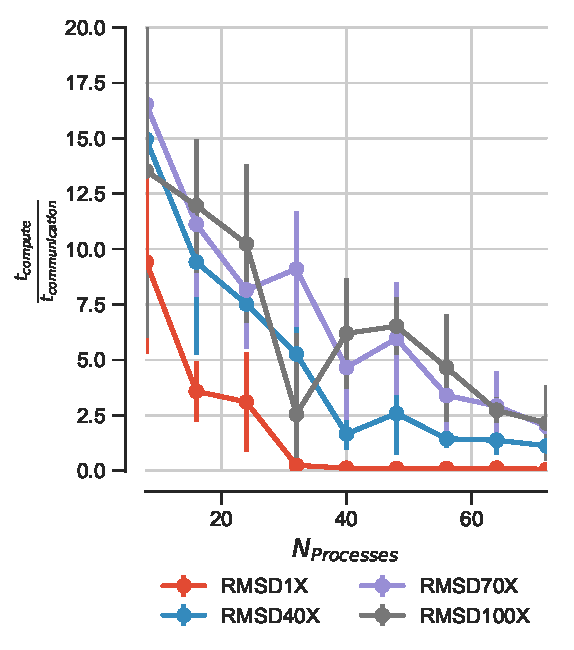
\includegraphics[width=\linewidth]{figures/Compute_to_comm_ratio_on_performance_v17.pdf}
  \captionsetup{format=hang}
\caption{Compute to communication ratio}
\label{fig:tcomp_tcomm_ratio}
\end{subfigure}
\hfill
\begin{subfigure}{.4\textwidth}
  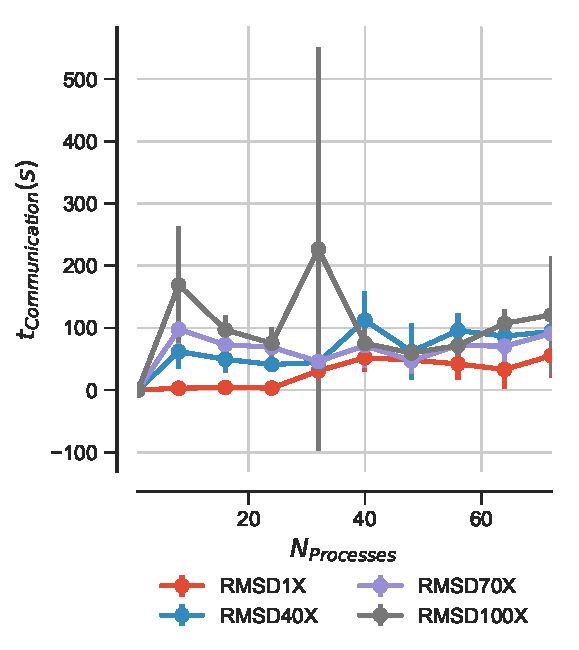
\includegraphics[width=\linewidth]{figures/comm_comparison_different_RMSD_overload.pdf}
  \caption{Communication time}
  \label{fig:MPItottime-chain-reader}
\end{subfigure}
\caption{(a) Change in compute to communication ratio with number of processes for different RMSD workload on SDSC Comet. 
(b) Comparison of communication time for different RMSD workload on SDSC Comet.
Five repeats were performed to collect statistics and error bars show standard deviation with respect to mean.}
\label{fig:tcom_tcomm_effect}
\end{figure}

\subsubsection{ChainReader}
In Section \ref{splitting-traj} we showed how splitting the trajectories would help to overcome I/O and improve scaling. 
However, the number of trajectories may not necessarily be equal to the number of processes.
For example, trajectories from MD simulations on HPC resources are often kept in small chunks and making sure that the number of processes is equal to the number of trajectory files will not be feasible for the typical users. 
The ChainReader, is used in \package{MDAnalysis} to represent multiple trajectories as one virtual trajectory. 
Here, we want to use ChainReader and measure its performance. 
In the current implementation of ChainReader, each process opens all the trajectories but I/O will only happen from a specific block of the trajectory specific to that process only.
 
 \begin{figure}[ht!]
\centering
\begin{subfigure}{.3\textwidth}
  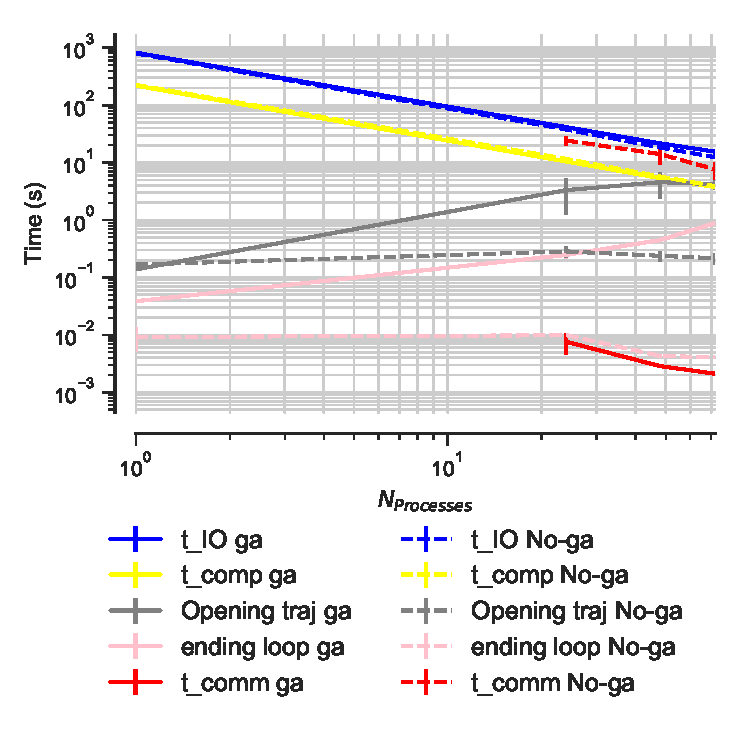
\includegraphics[width=\linewidth]{figures/Comparison_IO_compute_scaling_traj_splitting-chain-reader.pdf}
  \captionsetup{format=hang}
  \caption{Scaling for different components}
  \label{fig:MPIscaling-chain-reader}
\end{subfigure}
\hfill
\begin{subfigure}{.3\textwidth}
  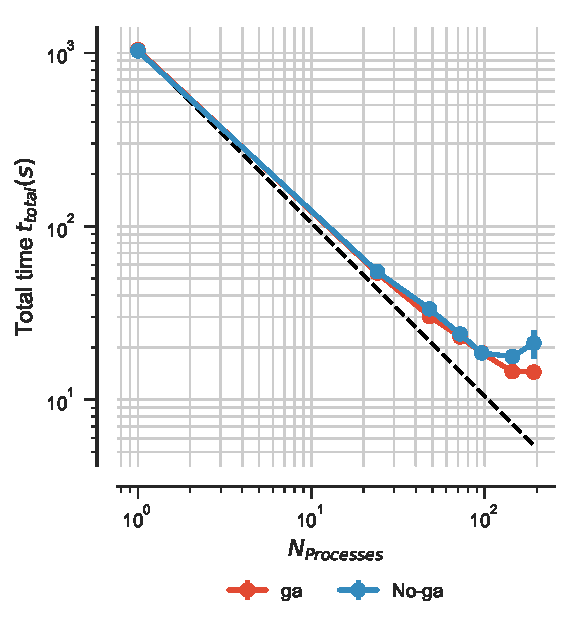
\includegraphics[width=\linewidth]{figures/Comparison_tot_time_traj_splitting-chain-reader.pdf}
  \caption{Scaling total}
  \label{fig:MPItottime-chain-reader}
\end{subfigure}
\hfill
\begin{subfigure}{.3\textwidth}
  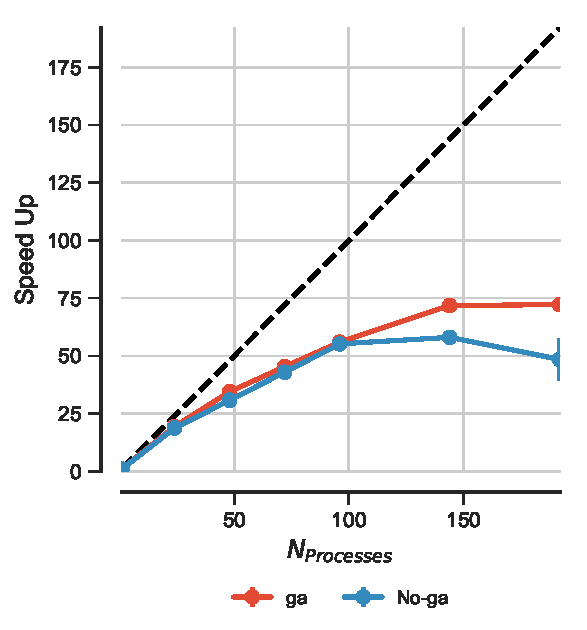
\includegraphics[width=\linewidth]{figures/Comparison_Speed_UP_traj_splitting-chain-reader.pdf}
  \caption{Speed-up}
  \label{fig:MPIspeedup-chain-reader}
\end{subfigure}
\bigskip

\begin{subfigure} {.45\textwidth}
  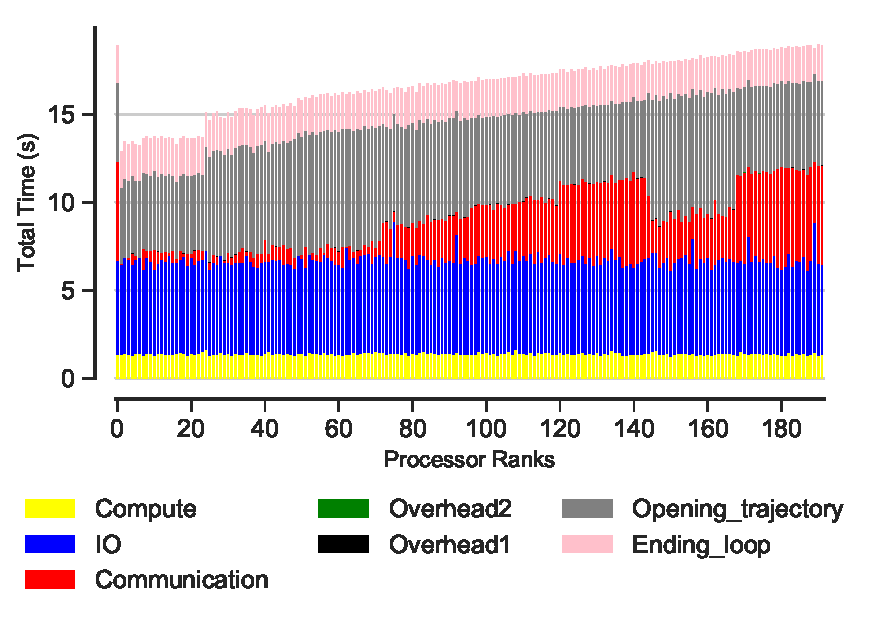
\includegraphics[width=\linewidth]{figures/chain-reader-no-ga-BarPlot-rank-comparison_192_5.pdf}
  \captionsetup{format=hang}
   \caption{Time comparison on different parts of the calculations per MPI rank using ChainReader without Global Arrays}
  \label{fig:MPIranks-split-chain-reader}
\end{subfigure}
\hfill
\begin{subfigure} {.45\textwidth}
  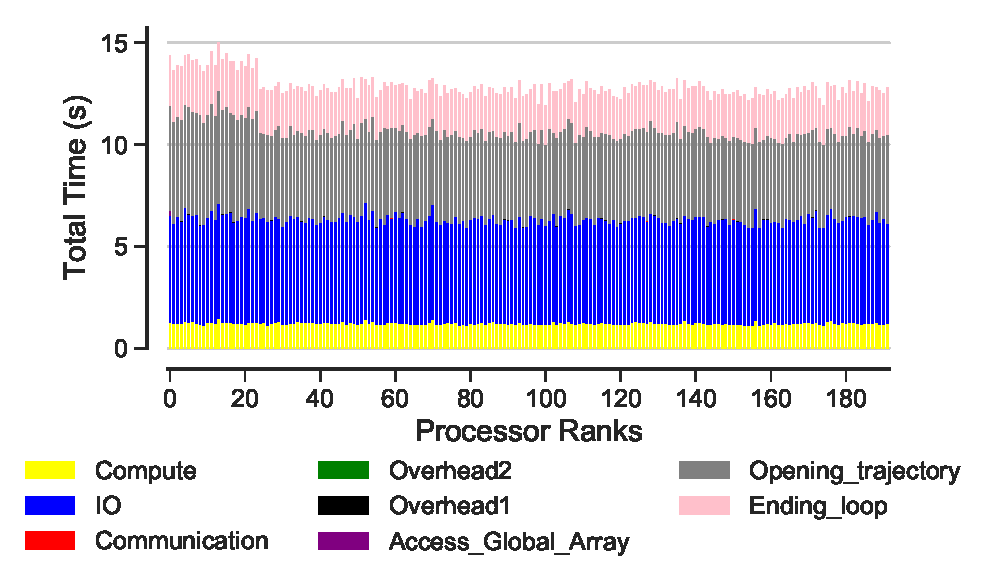
\includegraphics[width=\linewidth]{figures/chain-reader-ga-BarPlot-rank-comparison_192_3.pdf}
  \captionsetup{format=hang}
  \caption{Time comparison on different parts of the calculations per MPI rank using ChainReader using Global Arrays}
  \label{fig:MPIranks-split-ga-chain-reader}
\end{subfigure}

\caption{Comparison on the performance of ChainReader for RMSD task with MPI when the trajectories are split using Global Arrays and without Global Arrays ($\tcomp/\tIO \approx 0.3$) on SDSC Comet.
In case of Global Arrays, all ranks update the Global Arrays (\text{ga\_put()}) and rank 0 accesses the whole RMSD array through the global memory address (\text{ga\_get()}).
Five repeats were performed to collect statistics. (a) Compute \& I/O scaling versus number of processes (b) Total time scaling versus number of processes (c) Speed-up (a-c) The error bars show standard deviation with respect to mean. (d-e) Compute \tcomp, IO \tIO, communication \tcomm, access to the whole Global Arrays by rank 0 \text{$t_{\text{Access\_Global\_Array}}$}, ending the for loop \text{$t_{\text{end\_loop}}$},
  opening the trajectory \text{$t_{\text{opening\_trajectory}}$}, and overheads \text{$t_{\text{overhead1}}$}, \text{$t_{\text{overhead2}}$} per MPI rank (See Table \ref{tab:notation} for the definition). When Global Arrays is not used, the performance is affected due to the non-uniform communication time across different ranks. However, when Global Arrays is used communication time has significantly reduced and scaling is close to ideal. In addition, time for ending the for loop \text{t\_end\_loop} and 
opening the trajectory \text{$t_{\text{opening\_trajectory}}$} is a bottleneck as opposed to our calculation without ChainReader. We obtained the results for the ChainReader with a \emph{patched version} of the MDAnalysis that avoid race condition. \textbf{Note:} In serial, there is no communication.}
\label{fig:MPIwithIO-split-chain-reader}
\end{figure}

XDR based readers such as the reader for the XTC format that we use in this study store persistent offsets on disk \citep{Gowers:2016aa}. 
The offsets are used to enable access to random frames efficiently. 
The advantage of these offset files is that after opening the trajectory for the first time, opening the same file will be very fast afterward. 
These offsets will be generated automatically the first time the trajectory is opened and are stored in hidden $\ast.xtc\_offsets.npz$ files. 

It sometimes can happen that the stored offsets get out of sync with the trajectory they refer to. 
For this, the offsets also store the number of atoms, size of the file and last modification time. 
If any of these parameters change, the offsets are recalculated. 
If the XTC changes and any of the number of atoms, size of the file and last modification time changes but the offset file is not updated, then the offset file can be detected as invalid.
With ChainReader in parallel, each process opens all the trajectories; therefore in case of invalid offset file, several processes might want to recalculate these parameters and rebuild the offset file which will lead to race condition.
In order to avoid race condition, we removed this check from MDAnalysis, but this comes at the price of not checking the validity of the offset files at all; future versions of MDAnalysis will lift this limitation.
 
We obtained the results for the ChainReader with a \emph{patched version} of \package{MDAnalysis} that eliminates the race condition by assuming that XTC index files are present and valid. 
Figure \ref{fig:MPIwithIO-split-chain-reader} shows the results for performance of ChainReader for RMSD task using GA and without GA. 
As shown in Figure \ref{fig:MPIspeedup-chain-reader} the cases with GA and without GA scale up to 144 and 92 cores respectively.
The scaling is not close to ideal as opposed to what we achieved in Section \ref{splitting-traj}. 
However, in this case I/O and compute time are scaling very well (Figure \ref{fig:MPIscaling-chain-reader} as compared to Figure \ref{fig:ScalingComputeIO-split}) and the time for ending the for loop \text{$t_{\text{end\_loop}}$} (which includes the time for closing the trajectory file) and opening the trajectory \text{$t_{\text{opening\_trajectory}}$} appear to be the performance bottleneck as opposed to the results shown in Section \ref{splitting-traj} (i.e. Figures \ref{fig:MPIranks-split} and \ref{fig:MPIranks-split-ga}). 
One possible explanation for this behavior is because in ChainReader, each rank opens and closes all individual trajectory segments, i.e., for $N$ ranks and $M$ file segments, in total, $N M$ file opening/closing operations have to be performed. 
Each server that is part of a Lustre filesystem can only handle a limited number of I/O requests (read, write, stat, open, close, etc.) per second.
An excessive number of such requests, from one or more users and one or more jobs, can lead to contention for storage resources. 
For $N=M=100$, the Lustre file system has to perform 10,000 of these operations almost simultaneously, which might degrade performance. 
\obnote{Lustre will have to deal with ~10,000 file open and file close operations. Do we know its performance for file open/close?}
\mknote{This https://hpcf.umbc.edu/general-productivity/lustre-best-practices/ says that Opening a file keeps a lock on the parent directory. When many files in the same directory are to be opened, it creates contention. A better practice is to split a large number of files (in the thousands or more) into multiple subdirectories to minimize contention. It might be useful that put files in several subdirectories to avoid overhead}
 
\subsubsection{MPI-based Parallel HDF5}
\label{HDF5}
Another approach we examined to improve I/O scaling is MPI-based Parallel HDF5. 
We converted our XTC trajectory file into HDF5 format so that we can test the performance of parallel IO with HDF5 file format.
The code for this file format conversion can be found in the GitHub repository \url{https://github.com/hpcanalytics/supplement-hpc-py-parallel-mdanalysis}.
The time it took to convert our XTC file with $2,512,200$ frames into a simple custom HDF5 format was about $5400~s$ in our local resources with network file system (NFS).
We ran our benchmark on up to 8 nodes (192 cores) and, we observed near ideal scaling behavior with parallel efficiencies above 0.8 (Figure \ref{fig:comparison_efficiency} and Figures \ref{fig:MPIscaling-hdf5} and \ref{fig:MPIspeedup-hdf5}) with no straggler tasks (Figure \ref{fig:MPIranks-hdf5}).  
When we split our trajectory, scaling is better as compared to that of parallel I/O (Compare Figure \ref{fig:MPIspeedup-hdf5} to Figure \ref{fig:MPIspeedup-split}). 
However, both methods scale very well up to 8 nodes and have comparable performance.  

\begin{figure}[ht!]
\centering
\begin{subfigure}{.4\textwidth}
  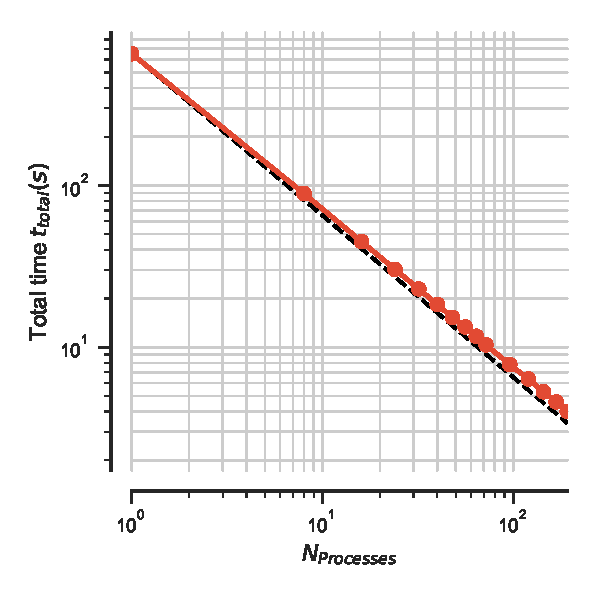
\includegraphics[width=\linewidth]{figures/hdf5-t_total.pdf}
  \caption{Scaling total}
  \label{fig:MPIscaling-hdf5}
\end{subfigure}
\hfill
\begin{subfigure}{.4\textwidth}
  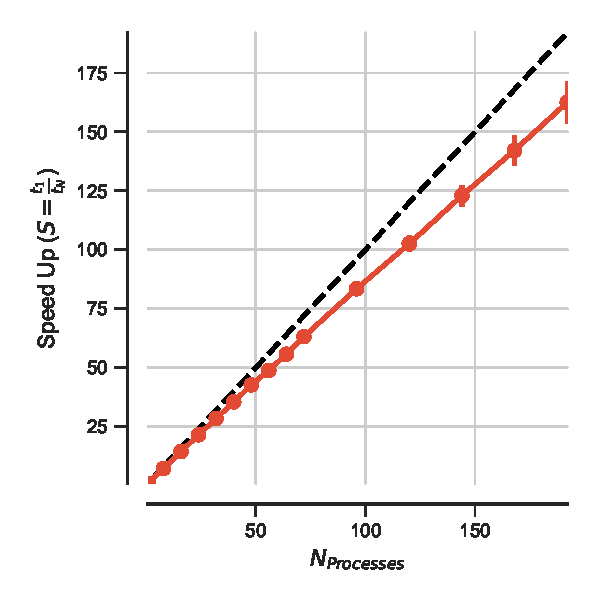
\includegraphics[width=\linewidth]{figures/hdf5-speed_up.pdf}
  \caption{Speed-up}
  \label{fig:MPIspeedup-hdf5}
\end{subfigure}
\bigskip

\begin{subfigure}{.4\textwidth}
\centering
  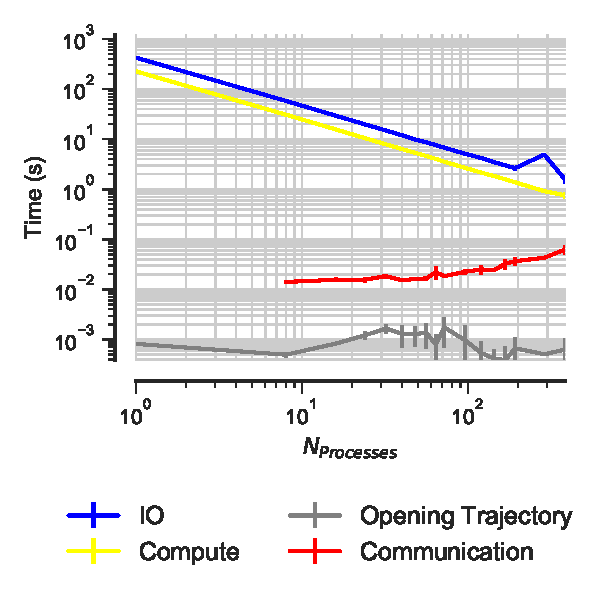
\includegraphics[width=\linewidth]{figures/hdf5-time_comp_IO_comparison.pdf}
  \captionsetup{format=hang}
\caption{Scaling for different components}
\label{fig:ScalingComputeIO-hdf5}
\end{subfigure}
\hfill
\begin{subfigure} {.5\textwidth}
  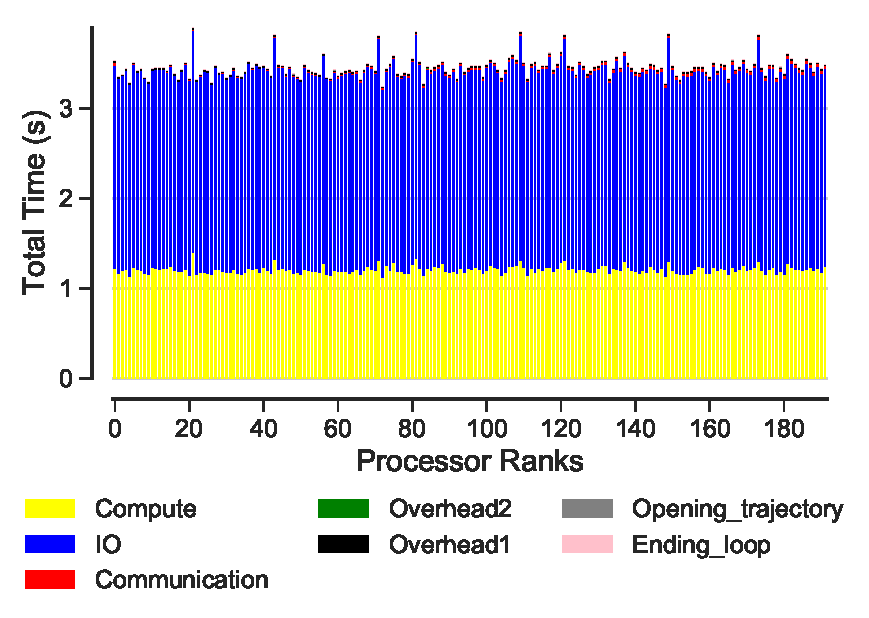
\includegraphics[width=\linewidth]{figures/hdf5-BarPlot-rank-comparison_192_4.pdf}
  \captionsetup{format=hang}
  \caption{Time comparison on different parts of the calculations per MPI rank}
  \label{fig:MPIranks-hdf5}
\end{subfigure}
%
\caption{Performance of the RMSD task with MPI-based parallel HDF5 (\text{$\tcomp/\tIO \approx 0.3$}) on SDSC Comet.
Data are read from the file system from a shared HDF5 file format instead of XTC format (Independent I/O) and results are communicated back to rank 0 (communications included). 
Five repeats were performed to collect statistics. (a-c) The error bars show standard deviation with respect to mean. (d) Compute \tcomp, IO \tIO, communication \tcomm, ending the for loop \text{$t_{\text{end\_loop}}$},
  opening the trajectory \text{$t_{\text{opening\_trajectory}}$}, and overheads \text{$t_{\text{overhead1}}$}, \text{$t_{\text{overhead2}}$} per MPI rank (See Table \ref{tab:notation} for the definition).
  This is typical data from one run of the 5 repeats. No straggler is observed. \textbf{Note:} In serial, there is no communication. I am reporting the slowest rank per timing, and that is averaged over all repeats.}
\label{fig:MPIwithIO-hdf5}
\end{figure}
